% Compile with XeLaTeX or LuaLaTeX
\documentclass[12pt]{report}
\usepackage[tmargin=1in,bmargin=1in,lmargin=1.25in,rmargin=1.25in]{geometry}
\usepackage{fontspec}
\usepackage{xcolor}
\usepackage{titlesec}
\defaultfontfeatures{Ligatures=TeX}
% Set sans serif font to Calibri
\setsansfont{Calibri}
% Set serifed font to Cambria
\setmainfont{Cambria}
% Define light and dark Microsoft blue colours
\definecolor{MSBlue}{rgb}{.204,.353,.541}
\definecolor{MSLightBlue}{rgb}{.31,.506,.741}
% Define a new fontfamily for the subsubsection font
% Don't use \fontspec directly to change the font
\newfontfamily\subsubsectionfont[Color=MSLightBlue]{Times New Roman}
% Set formats for each heading level
\titleformat*{\chapter}{\large\bfseries\sffamily\color{MSBlue}}
\titleformat*{\section}{\large\bfseries\sffamily\color{MSBlue}}
\titleformat*{\subsection}{\large\bfseries\sffamily\color{MSLightBlue}}
\titleformat*{\subsubsection}{\itshape\subsubsectionfont}

%For inserting Python Code
	\usepackage{listings}
	\usepackage{color}
	\definecolor{dkgreen}{rgb}{0,0,0}
	\definecolor{gray}{rgb}{0,0,0}
	
	
	\definecolor{mauve}{rgb}{0,0,0}
	\lstset{ %
	language=Python, % the language of the code
	basicstyle=\small, % the size of the fonts that are used for the code
	%numbers=left, % where to put the line-numbers
	%numberstyle=\tiny\color{gray}, % the style that is used for the line-numbers
	stepnumber=1, % each line is numbered
	numbersep=12pt, % how far the line-numbers are from the code
	backgroundcolor=\color{white}, % choose the background color. You must add \usepackage{color}
	showspaces=false, % show spaces adding particular underscores
	showstringspaces=false, % underline spaces within strings
	showtabs=false, % show tabs within strings adding particular underscores
	%frame=single, % adds a frame around the code
	rulecolor=\color{black}, % if not set, the frame-color may be changed on line-breaks within not-black text (e.g. commens (green here))
	tabsize=2, % sets default tabsize to 2 spaces
	captionpos=b, % sets the caption-position to bottom
	breaklines=true, % sets automatic line breaking
	breakatwhitespace=false, % sets if automatic breaks should only happen at whitespace
	%title=\lstname, % show the filename of files included with \lstinputlisting;
	% also try caption instead of title
	keywordstyle=\color{dkgreen}, % keyword style
	commentstyle=\color{dkgreen}, % comment style
	stringstyle=\color{dkgreen}, % string literal style
	escapeinside={\%*}{*)}, % if you want to add a comment within your code
	morekeywords={*,...} % if you want to add more keywords to the set
	}
	
	%%%%For inserting Python Code Ove
	
	
	
	%%%%%%%%%%%%%%%%%


\begin{document}
\section{A section}
This is some text.
\subsection{A subsection}
\subsubsection{A subsubsection}

\chapter{ Introduction}
	Treasure Hunt is a real-world, outdoor treasure hunting game using GPS-enabled devices. Participants navigate to a specific set of GPS coordinates and then attempt to find the geocache (container) hidden at that location.At its simplest level, geocaching requires these 8 steps:
	\begin{itemize}
	
	
	
	  \item Register with the game server.
	  \item Visit the "Hide & Seek a Cache" page.
	  \item Enter your name  and click "search."
	  \item Choose any Game Locations from the list and click on its name.
	  \item Click on Start Hunt from your Android  GPS Device.
	  \item Use yourAndroid  device to assist you in finding the hidden Treasure Location.
	   \item Share your Treasure Hunt stories and photos online.
	 
	\end{itemize}
	
	\section{Background}
	In the last few years, the smart phones (Android, Black 
	berry and iPhone) have taken over the market of Nokia 
	based Symbian Phones in India. And these smart phones 
	come equipped with A-GPS functionality which provides 
	the spatial coordinates of the user location. 
	Android's Network Location Provider determines user 
	location using cell tower and Wi-Fi signals, providing 
	location information in a way that works indoor and 
	outdoor, responds faster, and uses less battery power. 
	Assisted GPS [6], also known as A-GPS or AGPS, 
	improves the performance of standard GPS in devices 
	connected to the wireless network. A-GPS enhances the 
	location granularity of cell phones (and other connected 
	devices) in two ways: 
	
	\begin{itemize}
	\item By helping in finding a faster "time to first fix" 
	(TTFF). A-GPS acquires and stores information about 
	the location of satellites via the cellular network hence 
	the information does not need to be downloaded via 
	satellite
	\item By helping position mobile device when GPS signals 
	are not strong or not present. GPS satellite signals may 
	be impeded by tall towers, and they do not penetrate 
	building interiors well. A-GPS uses proximity to 
	cellular towers to calculate location when GPS signals 
	are unavailable. 
	\end{itemize}
	
	It addresses signal and wireless network problems by using 
	assistance from other services. Such a technology in our 
	smart phones can assist in various ways like tracking 
	current location, receiving turn-by-turn direction 
	instructions, route tracking, etc. Mostly suited for mobile devices, A-GPS takes assistance 
	from GPRS and at times, the service provider network 
	information, to pin-point the current location accurately. 
	Moreover the amount of CPU and programming required 
	for a GPS phone is reduced by diverting most of the work 
	to the assistance server instead. 
	
	A typical A-GPS enabled cell phone uses GPRS or other 
	such Internet based data connection to build a contact with 
	the assistance server for A-GPS. As this technique does 
	not take into account the cell phone service provider 
	network completely, we only pay for the GPRS usage 
	charges and nothing else. The only down-side to this 
	technology is that an A-GPS server cannot utilize any of 
	the three standby satellites available for GPS connections. 
	AGPS minimizes the amount of memory and hardware 
	that must be integrated into mobile devices in order to 
	provide GPS-quality device locating ability as required by 
	mobile devices. This keeps the mobile device simple and 
	allows longer battery time.
	
	GPS is real-time solution provider whereas AGPS is not. 
	The network usage is required every time we move out of 
	the service area. It is useful only for locating a particular 
	place in small area. There is no privacy in GPS and A-GPS 
	since the Assistance server knows the location of the 
	device. 
	
	There needs to be communication over the wireless for 
	processing of GPS information so this could be expensive
	
	\section{Implementation and Methodology}
	
	Location-based service is another key functionality that 
	gets used in smart phone applications. It is often combined 
	with maps to give a good experience to the user about their 
	location. 
	Android support LBS Application Programming Interfaces 
	(APIs) [7]. Location service allows finding out the device 
	current location. The application can request for periodic 
	update of the device location information. The application 
	can also register a intent receiver for proximity alerts like 
	when the device is entering and existing from an area of 
	given longitude, latitude and radius.
	
	

	
	
	
	\section{Designing Treasure Hunting Game}
	
	The executability of the activity should be concerned in designing Treasure Hunting Game. Therefore, the campus environment and local environment off the campus both can be adopted. The former is more suitable for beginners; the obvious buildings and landmarks in the campus, such as gate, playground, flower beds, gym, educational building, parking lot, etc can be the places for hiding the treasure. However, the safety should be concerned as well so that construction sites or some places with potential dangers should be avoided. In designing treasures, the treasure can be an object or the place itself. Once the participant is approaching the target, the system will automatically show the quiz. The quiz should be related to the treasure. For example, when the participant is approaching the flower bed, the system can appear “What kind of flower is it?” Thus, the participant needs to answer the question in this game. 
	
	Since the treasure hunting game integrates spatial map data, the system can display the places for the treasures according to the order you set. Also, the system can indicate the distance and the direction to the next scenic spot to clear up the participants’ confusion and to effectively mange the activity area and time (the figure below). As the treasure hunting game is finished, the system can automatically calculate the participants’ scores, which can be referred to how the students understand the quizzes. Also, you can apply other evaluation factors, such as answering time, the speed of finding the coordinates to be the evaluation criteria. Furthermore, the distance between each treasure should be designed carefully; neither too far nor too close is appropriate. If the distance is too close, it would be hard to tell how the students understand the quizzes; if the distance is too far, it would be difficult for the participants to find the direction to the next treasure.
	
	If the activity is held off the campus, the activity area should be concerned in designing the game. In general, public parks and scenic areas can be the activity area. If all of the conditions are met, the activity can be more flexible. For example, the participants can spend a half day finding the places of the treasures by bike. As a result, the activity area can be extended. Similarly, the rule of the game is to answer all of the questions in the system.
	
	No matter the activity area is in campus or off campus, the design of the questions should focus on the information which can be received by sensory organs. The questions for off-campus activities can be related to the local features, such as visiting historical sites of Qing Dynasty, seashore recreational route, historical architectures in old streets. On the other hand, the questions for the activities in campus can refer to the existing information in the campus, like the placard of flora and fauna, narration of special scenic spots, etc. The activity time can be decided by the number of treasures and the area of the activity, but it had better be less than four hours. If the time is too long, it might reduce students’ motivation of treasure hunting.
	
	
	
	
	
	
	\section{Proposed  System Advantages}
	In order to achieve this we are using the power of Open Source Android Operating System and Parse Cloud and APIOMAT API which has several benefits over other systems.Since we are using the cloud we have no bottle neck problem ,most of the code logic resides on the Parse
	and security model is not at all a problem anymore.Parse handles the security on the type of technology being used in the application like PHP,ANDROID,iOS all have different sets of Keys to access and manipulate the data.
	
	
	
	\begin{itemize}
	
	
	
	 \item No initial knowledge of Cloud Security Required
	\item Referencing the API will make the functionality easy
	\item  No Bottle Neck Problem 
	\item Executor Class for Sync data to web server in case of network not available
	\item Off Line Mode
	\item  disaster recovery
	\item Lower Maintenance  
	
	
	
	\end{itemize}
	
	
	
	
	\section{Locations & Rules }
	Geocaches can be found all over the world. It is common for geocachers to hide caches in locations that are important to them, reflecting a special interest or skill of the cache owner. These locations can be quite diverse. They may be at your local park, at the end of a long hike, underwater or on the side of a city street.In its simplest form, a cache always contains a logbook or logsheet for you to log your find. Larger caches may contain a logbook and any number of items. These items turn the adventure into a true treasure hunt. You never know what the cache owner or visitors to the cache may have left for you to enjoy. Remember, if you take something, leave something of equal or greater value in return. It is recommended that items in a cache be individually packaged in a clear, zipped plastic bag to protect them from the elements.
	
	People of all ages hide and seek geocaches, so think carefully before placing an item into a cache. Explosives, ammunition, knives, drugs and alcohol should not be placed in a cache. Respect local laws at all times.Please do not put food or heavily scented items in a cache. Animals have better noses than humans, and in some cases caches have been chewed through and destroyed because of food items in a cache.
	
	
	
	
	\section{Trackables}
	
	A Trackable is a sort of physical geocaching "game piece." You will often find them in geocaches or see them at geocaching gatherings. Each Trackable is etched with a unique code that can be used to log its movements on Geocaching.com as it travels in the real world. Some of these items have traveled hundreds of thousands of miles thanks to geocachers who move them from cache to cache!
	
	There are three main types of Trackables: Travel Bug® Track-ables, Geocoins and other Track-ables.A Travel Bug is a trackable tag attached to an item that geocachers call a "hitchhiker." Each Travel Bug has a goal set by its owner. Goals are typically travel-related, such as to visit every country in Europe or travel from coast to coast. Travel Bug Trackables move from cache to cache with the help of geocachers like you. See the "What do I do when I find a Trackable?" section of the guide for information on how you can help Trackables move.
	
	Geocoins are customizable coins created by individuals or groups of geocachers as a kind of signature item or calling card. They function exactly like Travel Bug Trackables and should be moved to another cache, unless otherwise specified by their owners.Other Trackable items come in various forms including patches, key rings and more. A common feature of Trackable items is that they bear a unique ID code and text noting that they are trackable at Treasure Hunt or Ankit APPS Google Play Store.
	
	
	\section{Conclusion}
	There are various constraints to implement Location Based 
	Services. The different kinds of constraints include 
	
	\begin{itemize}
	
	
	
	  \item Technology Constraints 
	For LBS to be operational on a large scale, mapping under 
	the geographical information system (GIS) needs to be 
	more comprehensive than it is today. This raises 
	significant challenges in for improving the breadth and the 
	depth of the existing coverage of GIS. The most important 
	factor in enabling the growth of LBS is wide availability of 
	cheap GPS enabled handsets. GPS enabled handsets are 
	being manufactured now days. The issue of cost remains to 
	be tackled, since these phones are still all high-end units
	
	\item Infrastructure Constraints 
	One of the main problems is the lack of spread of the 
	wireless network into the countryside. In developing 
	country like India, the wireless technology is in very 
	nascent stage. In metro cities and areas, the problem of 
	network congestion is also an important issue. The 
	percentage of service operators not meeting the congestion 
	rate benchmarks has risen substantially.
	
	\item Market failure 
	One of the main constraints to the provision of value added 
	services, in general, and LBS in particular, is the market 
	structure of the mobile industry and the failure to unleash 
	the forces of competition. A key essential need for LBS 
	provision needs cross-network connections to be seamless, 
	and the current practices go against a cooperative attitude 
	for LBS provision. 
	
	
	
	\end{itemize}
	
	
	
	
	
	

	\chapter{Requirement Engineering}
	
	
	
	
	\section{Hardware Requirement }
	
	The hardware requirements may serve as the basis for a contract for the implementation of the system and should therefore be a complete and consistent specification of the whole system. They are used by software engineers as the starting point for the system design. It should what the system do and not how it should be implemented.
	
	\begin{itemize}
	
	\item 600 MHz Processor
	\item AMR Architecture
	\item Capacitive Screen
	\item Proximity Sensor
	\item GPS Sensor
	\item Azimuth Sensor
	\item Gyroscope
	\end{itemize} 
	

	
	
	
	
	\section{Software Requirement }
	
	The software requirements document is the specification of the system. It should include both a definition and a specification of requirements. It is a set of what the system should do rather than how it should do it. The software requirements provide a basis for creating the software requirements specification.  It is useful in estimating cost, planning team activities, performing tasks and tracking the teams and tracking the team's progress throughout the development activity.
	
	\begin{itemize}
	
	\item Running Android 2.3 or above
	\item Device must not be rooted 
	\item Eclipse Indigo
	\item PHP 
	\item Mysql
	\item HeidSQL
	\item SQL Lite Browser
	\end{itemize}
	
	
	
	
	
	
	
	
	
	
	\section{Functional Requirement}
	In software engineering, a functional requirement defines a function of a software system or its component. A function is described as a set of inputs, the behavior, and outputs (see also software). Functional requirements may be calculations, technical details, data manipulation and processing and other specific functionality that define what a system is supposed to accomplish. Behavioral requirements describing all the cases where the system uses the functional requirements are captured in use cases.
	
	
	\section{Non Functional Requirements}
	Functional requirements are supported by non-functional requirements (also known as quality requirements), which impose constraints on the design or implementation (such as performance requirements, security, or reliability). Generally, functional requirements are expressed in the form "system must do requirement", while non-functional requirements are "system shall be requirement". The plan for implementing functional requirements is detailed in the system design. The plan for implementing non-functional requirements is detailed in the system architecture
	
	
	
	
	
	\section{Requirement}
	
	
	
	The Android software development kit (SDK) includes a comprehensive set of development tools. These include a debugger, libraries, a handset emulator based on QEMU, documentation, sample code, and tutorials. Currently supported development platforms include computers running Linux (any modern desktop Linux distribution), Mac OS X 10.5.8 or later, Windows XP or later. The officially supported integrated development environment (IDE) is Eclipse using the Android Development Tools (ADT) Plugin, though IntelliJ IDEA IDE (all editions) fully supports Android development out of the box, and NetBeans IDE also supports Android development via a plugin.[9] Additionally, developers may use any text editor to edit Java and XML files, then use command line tools (Java Development Kit and Apache Ant are required) to create, build and debug Android applications as well as control attached Android devices (e.g., triggering a reboot, installing software package(s) remotely).Enhancements to Android's SDK go hand in hand with the overall Android platform development. The SDK also supports older versions of the Android platform in case developers wish to target their applications at older devices. Development tools are downloadable components, so after one has downloaded the latest version and platform, older platforms and tools can also be downloaded for compatibility testing.
	
	Android applications are packaged in .apk format and stored under /data/app folder on the Android OS (the folder is accessible only to the root user for security reasons). APK package contains .dex files (compiled byte code files called Dalvik executables), resource files, etc.
	
	\subsection{Android Development Kit}
	
	
		The Android 3.1 platform (also backported to Android 2.3.4) introduces Android Open Accessory support, which allows external USB hardware (an Android USB accessory) to interact with an Android-powered device in a special "accessory" mode. When an Android-powered device is in accessory mode, the connected accessory acts as the USB host (powers the bus and enumerates devices) and the Android-powered device acts as the USB device. Android USB accessories are specifically designed to attach to Android-powered devices and adhere to a simple protocol (Android accessory protocol) that allows them to detect Android-powered devices that support accessory mode.
	
	
	
	
	\section{Software Tools}
	
	\subsection{Eclipse}
		Eclipse is a multi-language software development environment comprising a base workspace and an extensible plug-in system for customizing the environment. It is written mostly in Java. It can be used to develop applications in Java and, by means of various plug-ins, other programming languages including Ada, C, C++, COBOL, Fortran, Haskell, JavaScript, Perl, PHP, Python, R, Ruby (including Ruby on Rails framework), Scala, Clojure, Groovy, Scheme, and Erlang. It can also be used to develop packages for the software Mathematica. Development environments include the Eclipse Java development tools (JDT) for Java and Scala, Eclipse CDT for C/C++ and Eclipse PDT for PHP, among others.
	
	
	\subsection{System Architecture}
	
		The Eclipse Platform uses plug-ins to provide all functionality within and on top of the runtime system, in contrast to some other applications, in which functionality is hard coded. The Eclipse Platform's runtime system is based on Equinox, an implementation of the OSGi core framework specification.
		This plug-in mechanism is a lightweight software componentry framework. In addition to allowing the Eclipse Platform to be extended using other programming languages such as C and Python, the plug-in framework allows the Eclipse Platform to work with typesetting languages like LaTeX,[13] networking applications such as telnet and database management systems. The plug-in architecture supports writing any desired extension to the environment, such as for configuration management. Java and CVS support is provided in the Eclipse SDK, with support for other version control systems provided by third-party plug-ins.
		With the exception of a small run-time kernel, everything in Eclipse is a plug-in. This means that every plug-in developed integrates with Eclipse in exactly the same way as other plug-ins; in this respect, all features are "created equal".[citation needed] Eclipse provides plug-ins for a wide variety of features, some of which are through third parties using both free and commercial models. Examples of plug-ins include a UML plug-in for Sequence and other UML diagrams, a plug-in for DB Explorer, and many others.
		The Eclipse SDK includes the Eclipse Java development tools (JDT), offering an IDE with a built-in incremental Java compiler and a full model of the Java source files. This allows for advanced refactoring techniques and code analysis. The IDE also makes use of a workspace, in this case a set of metadata over a flat filespace allowing external file modifications as long as the corresponding workspace "resource" is refreshed afterwards.
		Eclipse implements widgets through a widget toolkit for Java called SWT, unlike most Java applications, which use the Java standard Abstract Window Toolkit (AWT) or Swing. Eclipse's user interface also uses an intermediate graphical user interface layer called JFace, which simplifies the construction of applications based on SWT.
	
	
 
   

\chapter{Database Design}

\section{Introduction}
Database design is the process of producing a detailed data model of a database. This logical data model contains all the needed logical and physical design choices and physical storage parameters needed to generate a design in a Data Definition Language, which can then be used to create a database. A fully attributed data model contains detailed attributes for each entity. 

	\section{System and Database Design}
	
	The database of treasure hunting game system contains three parts, treasure location database, map basic data, and quiz database. Since each treasure location has geographic coordinates, the quiz can automatically appear when the participant is approaching the treasure. The map basic data apply a desktop geographic information system, such as SuperGIS Desktop 2.2 as a platform for creating maps. Then, according to the activity areas, you need to create different maps; for example, the activity held in campus needs to create maps with main buildings, educational buildings, libraries, etc. For the off-campus activities, the maps with main landscapes, roads, rivers, etc are necessary.
	
	The number and levels of quizzes can be arranged by database, and the system can select the quizzes randomly. Therefore, each student might have different quizzes; various relevant quizzes can be designed for the same treasure location. Besides multiple choices, the question type can be fill-in questions with pictures; for example, the system displays the picture of the plants, and the students need to fill in the question.
	
	The set of Treasure Hunting Game adopts SuperGIS Mobile Engine 3, the mobile GIS application SDK (Software Development Kit) as the core object and applies the highly-flexible development mode and complete object controls of SuperGIS Mobile Engine 3 to assist developers in developing intuitive and desired game program.


\begin {table}[H]
\begin{center}
\begin{tabular}{ |l|l|l| }
  \hline
  \multicolumn{3}{|c|}{Question Table} \\
    \hline
  Column Name&Data Type& Length \\
  \hline

qNum&String.&255\\
qQuestion&String.&255\\
qanswer&String.&255\\
qpoints&String.&255\\
qStatus&String.&255\\
qlat&String.&255\\
qlon&String.&255\\
qhint&String.&255\\
  \hline
\end{tabular}
\caption {Question SQL Database} \label{tab:title}
\label{the-label-for-cross-referencing}
\end{center}
\end {table}


\begin {table}[H]
\begin{center}
\begin{tabular}{ |l|l|l| }
  \hline
  \multicolumn{3}{|c|}{ANR Timing} \\
    \hline
  Minimum Response Time &1000.&mili seconds\\
  \hline


Strict Mode & 0 & Disabled \\

  \hline
\end{tabular}
\caption {Application Not Responding Settings} \label{tab:title}
\label{the-label-for-cross-referencing}
\end{center}
\end {table}


\begin {table}[H]
\begin{center}
\begin{tabular}{ |l|l|l| }
  \hline
  \multicolumn{3}{|c|}{Hash Map Mapping} \\
    \hline
  Column Name&Data Type& Length \\
  \hline


id&long.&Integer.Valueof(String) \\
qNum&String.&Integer.Valueof(String)\\
qQuestion&String.&String.Valueof(String)\\
qanswer&String.&String.Valueof(String)\\
qpoints&String.&String.Valueof(String)\\
qStatus&String.&String.Valueof(String)\\
qlat&String.&Double.Valueof(String)\\
qlon&String.&Double.Valueof(String)\\
qhint&String.&String.Valueof(String)\\
  \hline
\end{tabular}
\caption {Hash Map Linked to Simple Adapter} \label{tab:title}
\label{the-label-for-cross-referencing}
\end{center}
\end {table}


\chapter{System Design}

\section{Data Flow Diagram}
A data flow diagram (DFD) is a graphical representation of the “flow” of data through an information system. It differs from the flowchart as it shows the data flow instead of the control flow of the program. A data flow diagram can also be used for the visualization of data processing. \\

\begin{figure}[ht!]
\left
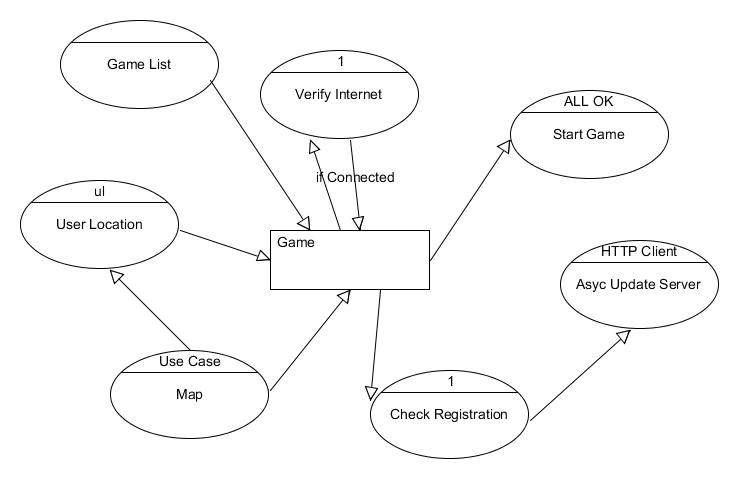
\includegraphics[width=150mm]{images/dfd0}
\caption{Dafa Flow Diagram 0}
\label{overflow}
\end{figure}
\newpage

\begin{figure}[ht!]
\left
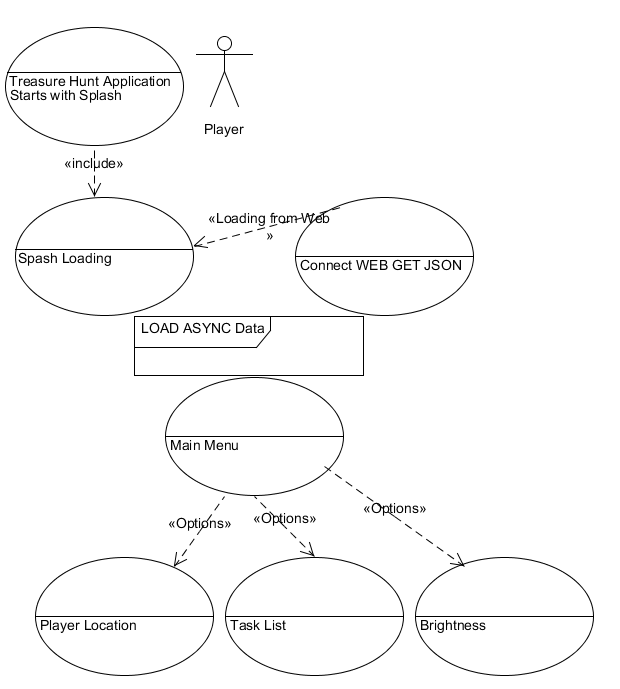
\includegraphics[width=150mm]{dfd0}
\caption{Dafa Flow Diagram 1}
\label{overflow}
\end{figure}
\newpage

\section{Sequence Diagram}
A sequence diagram in UML is a kind of interaction diagram that shows how processes operate with one another and in what order. \\

\begin{figure}[ht!]
\left
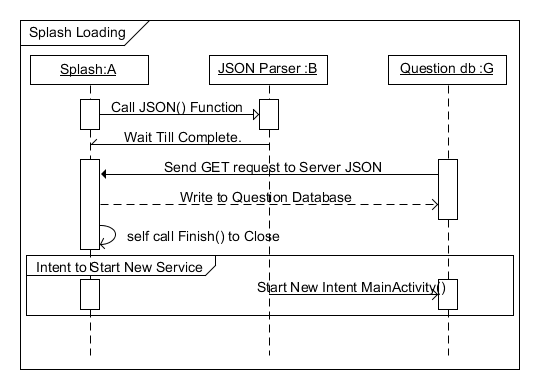
\includegraphics[width=150mm]{splash}
\caption{A simple Splash Screen Loading}
\label{overflow}
\end{figure}
\newpage


\section{Activity Diagram}
Activity diagram are a loosely defined diagram to show workflows of stepwise activities and actions, with support for choice, iteration and concurrency. UML, activity diagrams can be used to describe the business and operational step-by-step workflows of components in a system. 

\begin{figure}[ht!]
\left
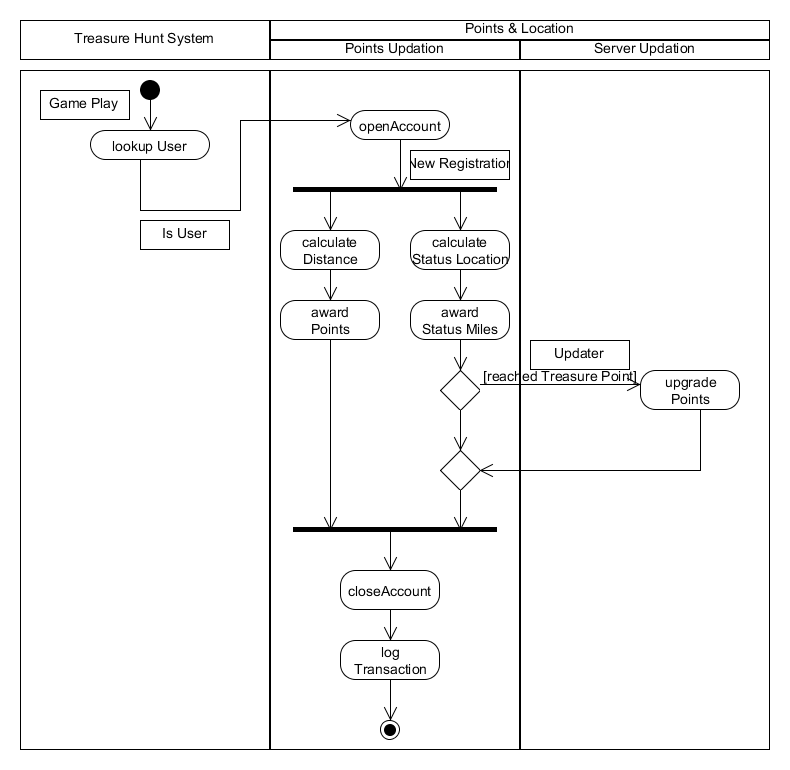
\includegraphics[width=150mm]{images/activityflow}
\caption{Game Checking Flow}
\label{overflow}
\end{figure}

\begin{figure}[ht!]
\left
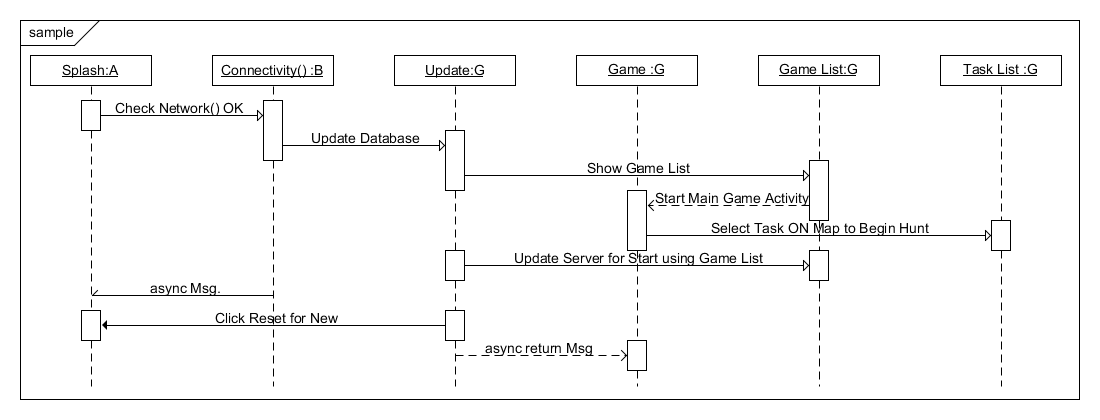
\includegraphics[width=150mm]{reset}
\caption{Game Activity Flow}
\label{overflow}
\end{figure}


\section{Use Case Diagram}
A use case diagram is a graph of actors, a set of use cases enclosed by a system boundary, communication (participation) association between the actors and the use cases, and generalization among the use cases. 

\begin{figure}[ht!]
\left
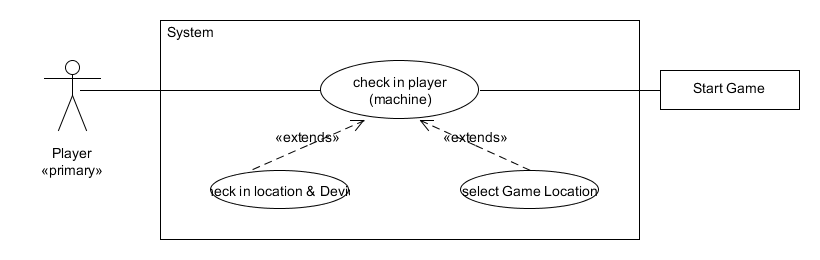
\includegraphics[width=150mm]{images/Usecases}
\caption{Use Case Diagram}
\label{overflow}
\end{figure}







\chapter{Input/Output Design}



\section{Input Design}
The input design is the link between the information system and the user. It comprises the developing specification and procedures for data preparation and those steps are necessary to put transaction data in to a usable form for processing can be achieved by inspecting the computer to read data from a written or printed document or it can occur by having people keying the data directly into the system. The design of input focuses on controlling the amount of input required, controlling the errors, avoiding delay, avoiding extra steps and keeping the process simple. The input is designed in such a way so that it provides security and ease of use with retaining the privacy. Input Design considered the following things:
\begin{itemize}
	
	

	
\item	What data should be given as input?
\item	 How the data should be arranged or coded?
\item	 The dialog to guide the operating personnel in providing input.
\item	Methods for preparing input validations and steps to follow when error occur.
 

\item	Input Design is the process of converting a user-oriented description of the input into a computer-based system. This design is important to avoid errors in the data input process and show the correct direction to the management for getting correct information from the computerized system.
\item It is achieved by creating user-friendly screens for the data entry to handle large volume of data. The goal of designing input is to make data entry easier and to be free from errors. The data entry screen is designed in such a way that all the data manipulates can be performed. It also provides record viewing facilities.
\item	When the data is entered it will check for its validity. Data can be entered with the help of screens. Appropriate messages are provided as when needed so that the user will not be in maize of instant. Thus the objective of input design is to create an input layout that is easy to follow.
\end{itemize}

\section{Output Design}
A quality output is one, which meets the requirements of the end user and presents the information clearly. In any system results of processing are communicated to the users and to other system through outputs. In output design it is determined how the information is to be displaced for immediate need and also the hard copy output. It is the most important and direct source information to the user. Efficient and intelligent output design improves the system’s relationship to help user decision-making.

	

\chapter{Modules}


\section{Module Description}
The modules functionality has been defined below with the snippets code

\subsection{Splash Startup}

A splash screen is an image that appears while a game or program is loading. It may also be used to describe an introduction page on a website. Splash screens cover the entire screen or simply a rectangle near the center of the screen. The splash screens of operating systems and some applications that expect to be run full-screen usually cover the entire screen.

Splash screens are typically used by particularly large applications to notify the user that the program is in the process of loading. They provide feedback that a lengthy process is underway. Occasionally, a progress bar within the splash screen indicates the loading progress. A splash screen disappears when the application's main window appears.
Splash screens typically serve to enhance the look and feel of an application or web site, hence they are often visually appealing. They may also have animations, graphics, and sound.

The Java programming language has a specific class for creating splash screens,  that handles standard splash screen functions, e.g. display an image centered on screen then disappears when the first program window opens.
Type the Code and Few lines here



\subsection{Async Task }

AsyncTask enables proper and easy use of the UI thread. This class allows to perform background operations and publish results on the UI thread without having to manipulate threads and/or handlers.

AsyncTask is designed to be a helper class around Thread and Handler and does not constitute a generic threading framework. AsyncTasks should ideally be used for short operations (a few seconds at the most.) If you need to keep threads running for long periods of time, it is highly recommended you use the various APIs provided by the java.util.concurrent pacakge such as Executor, ThreadPoolExecutor and FutureTask.

An asynchronous task is defined by a computation that runs on a background thread and whose result is published on the UI thread. An asynchronous task is defined by 3 generic types, called Params, Progress and Result, and 4 steps, called onPreExecute, doInBackground, onProgressUpdate and onPostExecute.

\lstinputlisting{async.py}

\subsection{JSON parser}

JSON (JavaScript Object Notation) is a lightweight data-interchange format. It is easy for humans to read and write.

 It is easy for machines to parse and generate. It is based on a subset of the JavaScript Programming Language, Standard ECMA-262 3rd Edition - December 1999. JSON is a text format that is completely language independent but uses conventions that are familiar to programmers of the C-family of languages, including C, C++, C#, Java, JavaScript, Perl, Python, and many others. These properties make JSON an ideal data-interchange language.

JSON is built on two structures:

\begin{description}
 \item[$\bullet$ ]  A collection of name/value pairs. In various languages, this is realized as an object, record, struct, dictionary, hash  table, keyed list, or associative array.
 \item[$\bullet$ ]  An ordered list of values. In most languages, this is realized as an array, vector, list, or sequence.

These are universal data structures. Virtually all modern programming languages support them in one form or another. It makes sense that a data format that is interchangeable with programming languages also be based on these structures.



\lstinputlisting{json.txt}

\end{description}
\subsection{SQL Lite Helper}
A helper class to manage database creation and version management.You create a subclass implementing onCreate (SQLiteDatabase), onOpen (SQLiteDatabase), and this class takes care of opening the database if it exists, creating it if it does not, and upgrading it as necessary. Transactions are used to make sure the database is always in a sensible state.This class makes it easy for ContentProvider implementations to defer opening and upgrading the database until first use, to avoid blocking application startup with long-running database upgrades.Exposes methods to manage a SQLite database.SQLiteDatabase has methods to create, delete, execute SQL commands, and perform other common database management tasks.See the Notepad sample application in the SDK for an example of creating and managing a database.Database names must be unique within an application, not across all applications
\lstinputlisting{sqllitehelper.py}

\subsection{GPS Receiver}

Android gives your applications access to the location services supported by the device through classes in the android.location package. The central component of the location framework is the LocationManager system service, which provides APIs to determine location and bearing of the underlying device (if available).As with other system services, you do not instantiate a LocationManager directly. Rather, you request an instance from the system by calling LOCATION_SERVICE.


\lstinputlisting{gps.py}


\subsection{Google Maps API}
With the Google Maps Android API, you can add maps to your app that are based on Google Maps data. The API automatically handles access to Google Maps servers, data downloading, map display, and touch gestures on the map. You can also use API calls to add markers, polygons and overlays, and to change the user's view of a particular map area.

The key class in the Google Maps Android API is MapView. A MapView displays a map with data obtained from the Google Maps service. When the MapView has focus, it will capture keypresses and touch gestures to pan and zoom the map automatically,including handling network requests for additional maps tiles. It also provides all of the UI elements necessary for users to control the map. Your application can also use MapView class methods to control the map programmatically and draw a number of overlays on top of the map.

The Google Maps Android APIs are not included in the Android platform, but are available on any device with the Google Play Store running Android 2.2 or higher, through Google Play services.
To integrate Google Maps into your app, you need to install the Google Play services libraries for your Android SDK..


	


\chapter{Testing}

\section{General}
The purpose of testing is to discover errors. Testing is the process of trying to discover every conceivable fault or weakness in a work product. It provides a way to check the functionality of components, sub assemblies, assemblies and/or a finished product. It is the process of exercising software with the intent of ensuring that the Software system meets its requirements and user expectations and does not fail in an unacceptable manner. There are various types of test. Each test type addresses a specific testing requirement.

\section{Developing Methodologies}
The test process is initiated by developing a comprehensive plan to test the general functionality and special features on a variety of platform combinations. Strict quality control procedures are used.The process verifies that the application meets the requirements specified in the system requirements document and is bug free. The following are the considerations used to develop the framework from developing the testing methodologies


\section{Robotium  benefits over other }

\begin{figure} [ht]
\centering

\includegraphics[scale=0.5]{robotinium}\\
\caption{Robotinium Automatic Application Testing Package }
\label{the-label-for-cross-referencing}
\end{figure}

\begin{itemize}
 \item You can develop powerful test cases, with minimal knowledge of the application under test.
 \item The framework handles multiple Android activities automatically.
 \item  Minimal time needed to write solid test cases.
 \item  Readability of test cases is greatly improved, compared to standard instrumentation tests.
 \item ] Test cases are more robust due to the run-time binding to GUI components.
 \item Blazing fast test case execution.
 \item Integrates smoothly with Maven or Ant to run tests as part of continuous integration.
\end{itemize}

\section{Results}
\begin{figure} [ht]
\centering
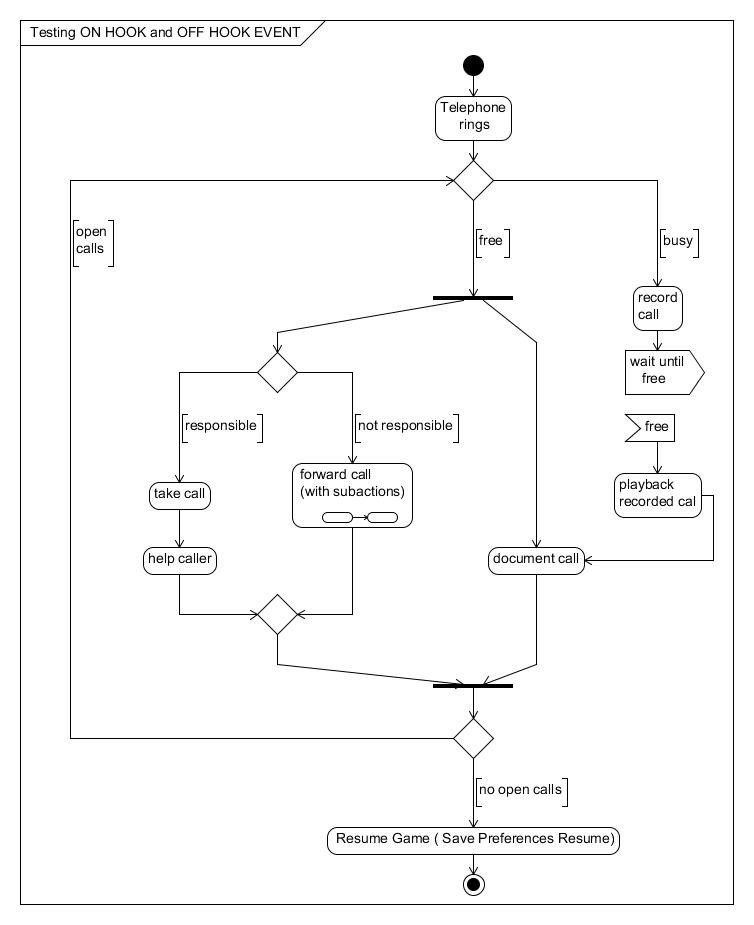
\includegraphics[scale=0.5]{testingcall}\\
\caption{Testing ON and OFF HOOK  }
\label{the-label-for-cross-referencing}
\end{figure}

\subsection{Analysis}
Code Snippet
\lstinputlisting{robotinium.py}



\chapter{Implementation}


\section{\ignorespacesSource Code & Screen Shots}

\subsection{Splash Screen}

\begin{wrapfigure}{r}{0.3845\linewidth}
\centering
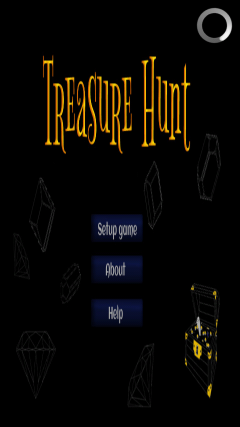
\includegraphics[scale=0.7]{snaps/splash}
\caption{Application Loading}
\label{fig:myfig}
\end{wrapfigure}
\textnormal{Splash Screen is a view that appears for sometimes (3 or 4 seconds).After dislaying splash screen that never comes second time in application until we restart Application.The purpose of a splash screen is to give the user an indication that your app is loading–not to create an extra delay before the user can load your app. People don’t like waiting, especially in a mobile environment.Using Thread,AsyncTask,Handler you can wait sometimes to load your app.The most desirable way to display splash screen is handler.you can do it easily.no need to create thread or async task in your activity.The handler have post Delayed (Runnable,long)  method.using this method you can wait some times to load app.Handler instance is associated with a single thread and that thread's message queue. When you create a new Handler, it is bound to the thread / message queue of the thread that is creating it -- from that point on, it will deliver messages and runnables to that message queue and execute them as they come out of the message queue.

}

\lstinputlisting{splash.py}



%\lstinputlisting{java/splash.java}


\subsection{Location Marker}

\begin{wrapfigure}{r}{0.39\linewidth}
\centering
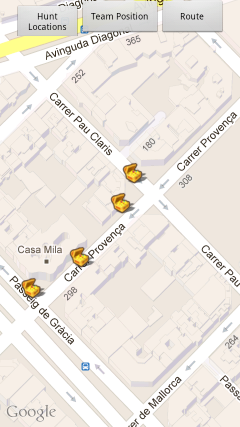
\includegraphics[scale=0.6]{snaps/location}
%\rule{0.9\linewidth}{0.75\linewidth}
\caption{Location Marker Activity}
\label{fig:myfig}
\end{wrapfigure}
\textnormal{
Location Marker is responsible  for plotting the real time location of all the user participating in the game. The functionality is when the player starts the application and registers it,the device starts sending the user co-ordinates to our webserver which is send back to other user using the JSON type in callback which uses the overlays on Android Maps to plot it.

In order to use the Android Maps you need to have maps and its API keys . The Treasure Hunt Icons are saved in the assets folder and the images are scaled for the device screen size and are in the PNG format.Using this Location Marker the user is not only able to see his locations but other locations where the other team are heading .

}

\lstinputlisting{showthemap.py}
%\lstinputlisting{java/LocationMarker.java}

\subsection{Task List}

Treasure Hunting Game not only remains the concept of hunting treasures with maps but also integrates GPS function. With a designed route for treasure hunting, the students would not miss any places for treasures. During the process of game, students can participate in the activity and observe the environment in person and absorb the knowledge unconsciously. Meanwhile, students can learn how to apply GPS and the skills of reading maps to obtain the knowledge happily.Treasure Hunting Game not only remains the concept of hunting treasures with maps but also integrates GPS function. With a designed route for treasure hunting, the students would not miss any places for treasures. During the process of game, students can participate in the activity and observe the environment in person and absorb the knowledge unconsciously. Meanwhile, students can learn how to apply GPS and the skills of reading maps to obtain the knowledge happily.

\begin{equation*}
  \begin{CD}
    a @>>> b \\
    @VVV @AAA \\
    c @= d
  \end{CD}
  \qquad
  \begin{CD}
    x @>>\alpha> y \\
    @VV\kappa V @A\beta AA \\
    v @<\gamma<< w
  \end{CD}

\end{equation*}

%\lstinputlisting{java/TaskList.java}


\subsection{User Registration}

Treasure Hunting Game can only be played when the user has registered with the server and his device IMSI has been saved on the server,Once the user Installs the Application the user is asked to register the device and select team color , this is achieved using the registration class . A seperate XML layout has been developed for the Registration form . Once the data has been saved the entry is created in Shared Preferences and the application sends the data to webserver , the type of data is UTF-8 and in JSON format

\begin{align*}
\xymatrix@R=10pt{
    cRing \ar[r] & Sch \\
    A \ar@{}[u]|{\rotatebox{90}{$\in$}} \ar@{|->}[r] 
            & Spec(A) \ar@{}[u]|{\rotatebox{90}{$\in$}}
}
\end{align*}



	
\chapter{Snapshot}

\begin{figure}[h]
\begin{center}$
\begin{array}{cc}
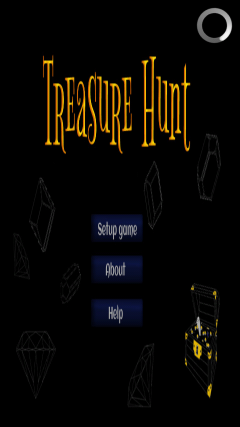
\includegraphics[width=2.5in]{snaps/splash} &
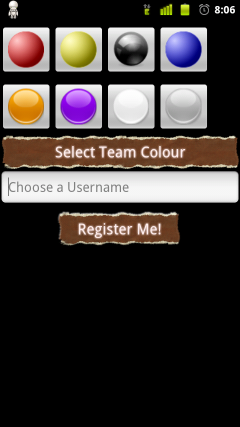
\includegraphics[width=2.5in]{snaps/user} &

\end{array}$
\end{center}
\caption{Spash Screen & Team Select}
\end{figure}

\begin{figure}[h]
\begin{center}$
\begin{array}{cc}
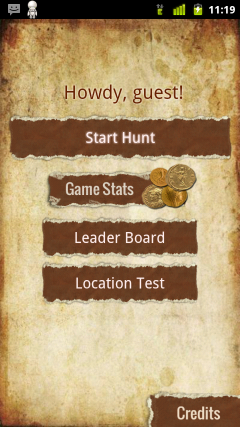
\includegraphics[width=2.5in]{snaps/3} &
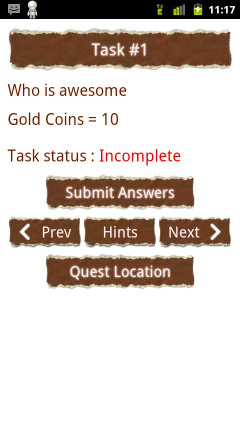
\includegraphics[width=2.5in]{snaps/4} 
\end{array}$
\end{center}
\caption{Main Menu & Task List}
\end{figure}

\begin{figure}[h]
\begin{center}$
\begin{array}{cc}
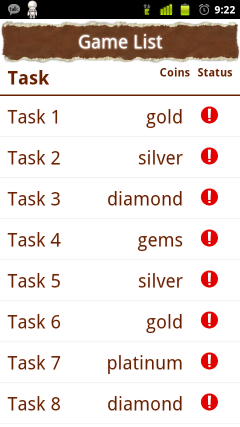
\includegraphics[width=2.5in]{snaps/5} &
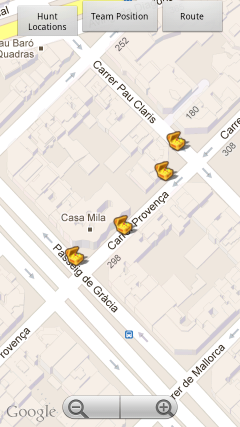
\includegraphics[width=2.5in]{snaps/6} 
\end{array}$
\end{center}
\caption{OverLays Map & Custom Location}
\end{figure}

\begin{figure}[h]
\begin{center}$
\begin{array}{cc}
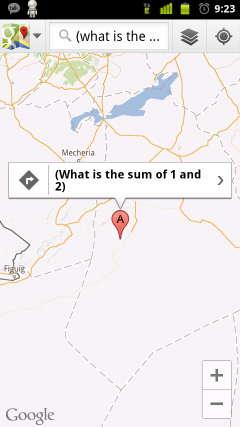
\includegraphics[width=2.5in]{snaps/7} &
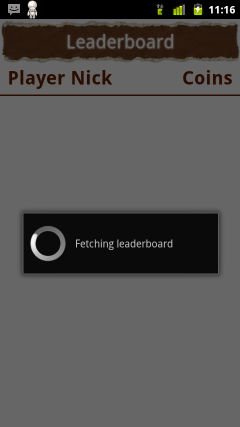
\includegraphics[width=2.5in]{snaps/8} 
\end{array}$
\end{center}
\caption{Async Loading using Simple Adapter}
\end{figure}

\begin{figure}[h]
\begin{center}$
\begin{array}{cc}
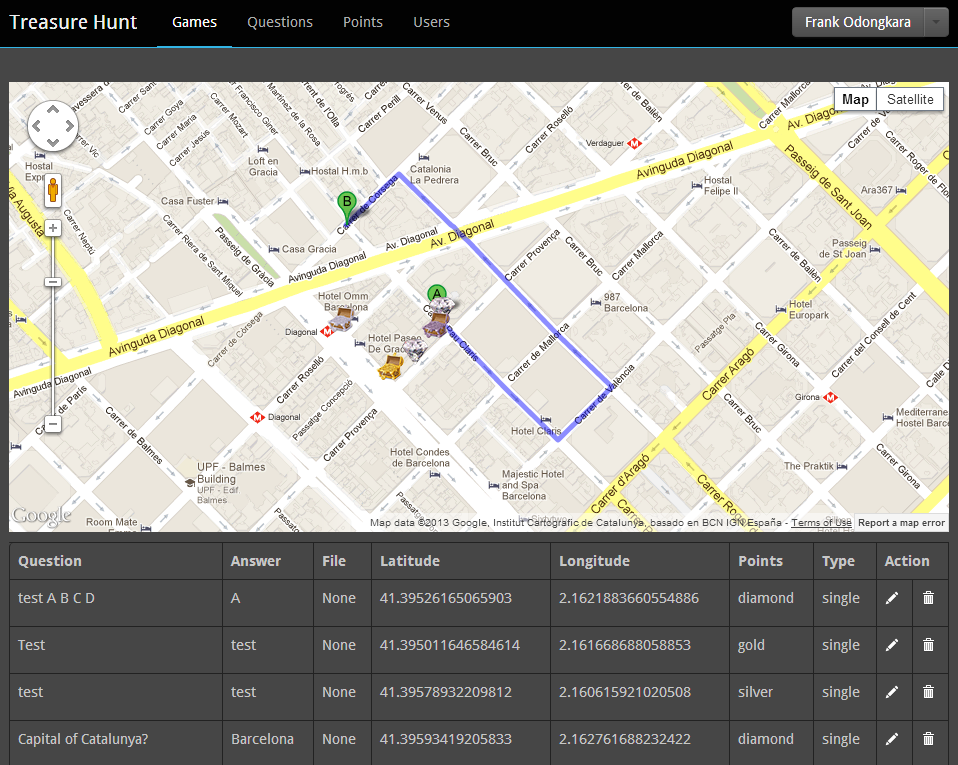
\includegraphics[width=2.5in]{images/maps} &
\end{array}$
\end{center}
\caption{Google Maps on Server }
\end{figure}




\chapter{Future Aspects}

Being build with the power of Cloud and Android this will have many uses , Its not long back when on April 1 2013 Google Released location where actual treasures were found by treasure hunters where other native people considered that as a April fools day Ha-ox. Implementing In Video on Google Customized Maps over Overlays and Custom route navigation with intelligent navigation is what will be released in the next release . The Application can be found on Google Play under the name of Treasure Hunt [Ankit APPS] \\

\chapter{Conclusion}

Treasure Hunting Game not only remains the concept of hunting treasures with maps but also integrates GPS function. With a designed route for treasure hunting, the students would not miss any places for treasures. During the process of game, students can participate in the activity and observe the environment in person and absorb the knowledge unconsciously. Meanwhile, students can learn how to apply GPS and the skills of reading maps to obtain the knowledge happily.








\end{adjustwidth}



\end{document}